\chapter{MeVガンマ線天文学}
現在の天文学において、宇宙は電波・赤外線・X線といった様々な領域にわたる波長での観測が行われている。その中でもサブMeV$\sim$数十MeV領域の宇宙ガンマ線を観測することでブラックホール・活動銀河核・宇宙線起源・超新星爆発といった事象の解明が可能になると考えられている。
\section{これまでのMeVガンマ線天文学}
\subsection{MeVガンマ線領域}

画像だよ画像だよ画像だよ画像だよ画像だよ画像だよ画像だよ画像だよ画像だよ画像だよ画像だよ画像だよ画像だよ画像だよ画像だよ画像だよ画像だよ画像だよ画像だよ画像だよ画像だよ画像だよ画像だよ画像だよ画像だよ画像だよ画像だよ画像だよ画像だよ画像だよ画像だよ画像だよ画像だよ画像だよ画像だよ画像だよ画像だよ画像だよ画像だよ画像だよ画像だよ画像だよ画像だよ画像だよ画像だよ画像だよ画像だよ画像だよ画像だよ画像だよ画像だよ画像だよ画像だよ画像だよ画像だよ画像だよ画像だよ画像だよ画像だよ画像だよ画像だよ画像だよ画像だよ画像だよ画像だよ画像だよ画像だよ画像だよ画像だよ画像だよ画像だよ画像だよ画像だよ画像だよ画像だよ画像だよ画像だよ画像だよ画像だよ画像だよ画像だよ画像だよ画像だよ画像だよ画像だよ画像だよ画像だよ
\begin{figure}
\centering
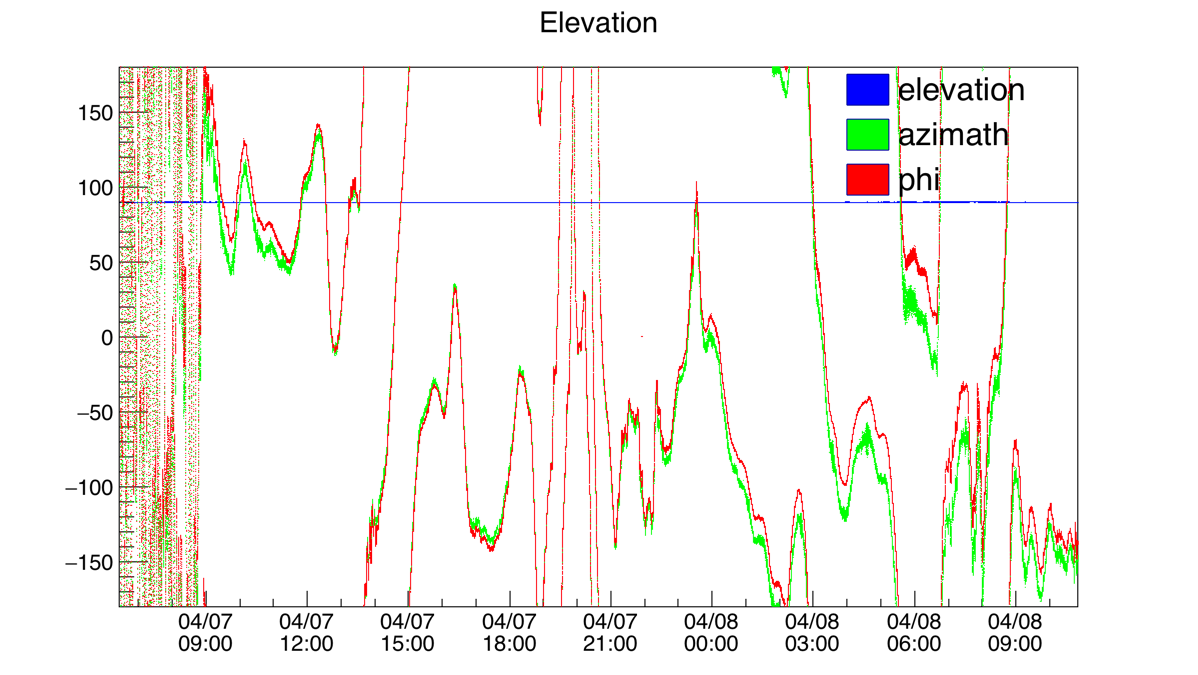
\includegraphics[width=15cm]{attitude_f.png}
\caption{test}
\end{figure}
